\chapter{Background}
	
	\label{sec:background}
	
	This chapter aims to familliarise the reader with the principles of neural
	modelling and the challenges involved in simulating these models at biological
	scales and speeds. An overview is given of the current state-of-the-art of
	supercomputer technology and their suitability for neural modelling. This is
	followed by an introduction to specialised `neuromorphic' systems which
	specifically target neural simulation tasks and overcome the limitations of
	current supercomputers. Finally, the chapter covers the interconnection
	network of SpiNNaker, a neuromorphic platform which will form a platform for
	the work proposed later in this report.
	
	\section{Modelling the brain}
		
		% What is done, for what purpose
		
		The brain is an extremely complex and variable organ whose high-level
		behaviours are similarly complex and variable. Unsurprisingly, efforts to
		understand the brain, rely heavily on simplified models of its function and
		implementation. Modelling approaches cover a wide spectrum from extremely
		detailed models of the neurophysiology of individual neurons
		\cite{carnevale06} to high level models where mathematical functions are
		mapped automatically onto large populations of neurons \cite{eliasmith04}.
		This report focuses towards the latter end of the spectrum. This section
		gives a brief historical context for the modelling approaches in use today
		followed by an overview of the NEF, a high-level modelling framework to give
		a feel for the way networks are built.
		
		\subsection{History of neural modelling}
			
			The development of high-level neural models can be divided up into three
			coarse generations, each increasing their level of biological realism
			\cite{vainbrand11}.
			
			The first generation of models, such as the McCulloch-Pitts threshold neuron
			\cite{mcculloch43}, consisted of testing if a simple, linear function of
			the neuron's inputs was above a threshold value and outputting either a
			`high' or `low' signal. The function used in each neuron and the pattern
			of connectivity in the network define the behaviour of the network as a
			whole.
			
			It was noted that communication between biological neurons was not simply
			level-based but instead appeared to be based on the rate at which
			electrical `spikes' were emitted (or `fired') by neurons to their
			neighbours. The second generation sought to model this by representing the
			output of a neuron as a continuous value \cite{maass97}. Once again, the
			network's behaviour was defined by the functions computed by each neuron
			and the network's connectivity.
			
			\begin{figure}
				\center
				\input{|"python2 figures/snn-example.py"}
				\caption{Simple leaky-integrate-and-fire neuron example.}
				\label{fig:snn-example}
			\end{figure}
			
			The third generation of extended the idea further noting that the firing
			rate is not the only significant factor but also that the timing of spikes
			is significant too \cite{maass01}. As a result, neural models were devised
			that modelled some of the physiological properties of neurons.
			
			The level of biological detail of such models varies greatly but many
			models build on the `leaky integrate and fire' (LIF) model.  Spikes
			arriving at a LIF neuron cause a temporary flow of current into or out of
			the neuron, modelling the behaviour of synapses in biological neurons. The
			LIF neuron integrates this current over time, accumulating charge which
			gradually leaks away over time. If the charge in the neuron reaches a
			certain threshold, it produces a spike and its charge is reset. This
			process is illustrated in figure \ref{fig:snn-example}.
			
			One of the key parameters of a neural network is the amount of influence
			each incoming spike has on a neuron. Typically, this influence is modelled
			by assigning a weight to each synapse which scales the impact of a spike
			arriving via that synapse. As with the exact behaviour of the neurons
			themselves, key modelling task is appropriately selecting these weights.
			
			Models of many types of learning in the brain revolve around modelling the
			self-adjustments of these weights by the brain. The exact rules by which
			these weights are adjusted is the subject of much active research though
			most promising approaches attempt to learn from the relative timing
			\cite{pfister06} or rate \cite{bienenstock82} of spikes arriving at a
			neuron. As well as adjusting weights, some learning rules can also form
			entirely new connections between previously disconnected neurons
			\cite{bamford10}.
		
		\subsection{High-level modelling}
			
			The Neural Engineering Framework (NEF) \cite{eliasmith04} is a high level
			framework for constructing large neural models which exhibit complex,
			high-level behaviours. The NEF has been used to build large, complex
			models including Spaun as described in \emph{`How to build a brain'},
			(Eliasmith, 2013) \cite{eliasmith13}. The key to the NEF's ability to
			model complex behaviours is its high-level approach to neural network
			design. This high-level approach is based on three `principles' which are
			enumerated below:
			
			\begin{description}
				
				\item[Representation] The spiking activity of a population of simple
				neuron models encode vectors (i.e. an array of numerical values).
				
				\item[Transformation] Arbitrary mathematical functions can be computed
				by selecting appropriate connection weights between populations of
				neurons representing input values and a target population which will
				represent the result.
				
				\item[Dyanmics] By connecting populations of neurons back to themselves,
				a control system is formed which can be tuned to produce interesting
				dynamical behaviour. This can be used, for example, as a basis for
				working memory.
				
			\end{description}
			
			By applying these principles, the NEF can be considered analogous to a
			compiler for neural models. An implementation of the NEF for the Python
			programming language called Nengo has been produced which enables users to
			literally describe functions in standard Python code which are then
			directly `compiled' into a neural model. Using this system, `Libraries' of
			useful neural models and subcomponents have been built. A prominent
			example is the Semantic Pointer Architecture (SPA) \cite{eliasmith13}
			which provides additional higher level features including a symbolic
			representation system.
		
	
	\section{Simulating brains}
		
		The range of neural models described in the previous section all present a
		significant computational challenge it simulate at scale. This section
		briefly outlines the challenges faced when simulating large models.
		
		% TODO Introduce
		
		\subsection{Computation}
			
			Computationally, spiking neural models can be relatively simple, the state
			of the neuron is described by a differential equation over time. Neuron
			states are typically updated with a fairly coarse granularity of once per
			0.1 to 1.0 ms. Additional calculations are also required to update the
			neurons' states upon spike arrival. In the case of networks featuring
			learning models, spike arrivals also typically entail further calculations
			in order to update weights.
			
			Given that the human brain contains around 100 billion ($10^9$) neurons
			each with around 10,000 synapses, this constitutes a non-trivial amount of
			of computation. In order to maintain real-time performance, the simulation
			of different neurons must be distributed across a large number of
			processing cores.
		
		\subsection{Communication}
			
			% Number of spikes produced, the form that spikes take, multicast,
			% possible changes due to learning. Especially fun for real-time.
			
			% spiking at an average rate of 10 Hz
			
			The feature of neural models which stresses simulators most, however, is
			their communications requirements. Since neurons in the brain fire at an
			average rate of around 10 Hz in a human-sized model, 100 trillion
			($10^{14}$) spikes must be delivered within a model every second. Since
			neurons connect to around 10,000 others, their spikes need to be
			transmitted to a large number of destinations. Unfortunately, conventional
			computer networks tend to be focused on supporting efficient one-to-one
			(unicast) connectivity. In many cases meaning that each spike must be
			repeatedly transmitted, once for each destination, which costs both large
			amounts of network resource and consequently large amounts of power. To
			achieve greater efficiency, multicast communications can be used where the
			message is sent once and is delivered to multiple locations and only
			duplicated within the network at the latest possible moment.
			
			An additional challenge for interconnection models is the amount of data
			involved in individual communications within neural simulators. Spike
			messages encode only a very limited amount of data: their source neuron
			and the time they were produced. This means that individual messages sent
			through the network tend to be very small even though the aggregate
			network utilisation may be high. This pattern is directly opposed to many
			conventional computational problems which instead tend to transmit large,
			continuous blocks of data at more infrequent intervals. As a result,
			conventional networks can impose large overheads when dealing with spikes
			due to their small size. Some researchers have experimented with sending
			many spikes at once in order to reduce the overhead involved however the
			effectiveness of this technique can be limited in certain models
			\cite{morrison05}.
			
			Luckily, much of the connectivity within the brain is highly local meaning
			that neurons tend to mostly connect to physically nearby neurons. This
			type of predominantly local communication is well supported by most
			scalable computer networks such as those found in supercomputers. In order
			to take advantage of this property, however, models must be carefully laid
			out within a simulator's network. This problem known to be NP-complete
			though effective heuristics solutions are known to exist \cite{haldar00}.
		
		
	
	\section{Supercomputer technology}
		\label{sec:supercomputers}
		
		\begin{table}
			\center
			\begin{tabular}{r l r r r l l l}
				\toprule
				Rank & Name    & Pflops& Cores  & Nodes  & Topology & Interconnect          & Sources \\
				\midrule                          
				1 & Tianhe-2   & 33.86 & 3,120,000 & 16,000 & Fat-Tree & Electrical \& Optical & \cite{dongarra13} \\
				2 & Titan      & 17.59 & 560,640   & 18,688 & 3D Torus & Electrical            & \cite{bland12} \\
				3 & Sequoia    & 17.17 & 1,572,864 & 98,304 & 5D Torus & Electrical \& Optical & \cite{prickett10} \\
				4 & K Computer & 10.51 & 705,024   & 68,544 & 6D Torus & Electrical            & \cite{fujitsu11,yokokawa11} \\
				5 & Mira       &  8.59 & 786,432   & 49,152 & 5D Torus & Electrical \& Optical & \cite{prickett10} \\
				\bottomrule
			\end{tabular}
			
			\caption{Top Five `Top500' Supercomputers, June 2014.}
			\label{tab:top500}
		\end{table}
		
		The Top500 list \cite{meuer14j} aims to enumerate, biannually, the 500
		fastest supercomputers in the world ranked by their performance on the
		LINPACK benchmark \cite{dongarraLINPAC}. The list offers an insight into the
		current state-of-the-art for high-performance computing. Table
		\ref{tab:top500} shows the top five machines in the Top500 list released in
		June 2014 along with basic details of the type of interconnection involved.
		In this section an overview is given of the architecture of these large
		scale machines.
		
		The LINPACK benchmark performs computations to ``analyze and solve linear
		equations and linear least-squares problems'' to produce a computational
		load representative of certain computational tasks common to scientific
		computing \cite{dongarra84}. In particular it is a CPU-bound problem which
		attempts to measure the peak CPU performance achievable\footnote{Where CPU
		Performance is measured in Petaflops: how many quadrillion ($10^{15}$)
		floating point operations can be performed per second.} but without any
		significant indication of the performance of the network which connects the
		system together \cite{dongarra07}.
		
		Since simulation of spiking neural networks requires a large amount of
		communication but relatively small amounts of computation, this benchmark is
		clearly not representative of the workload of such a task.  In fact, many
		modern supercomputer workloads also rely on network performance to a
		greater degree than the LINPACK benchmarks and as a result a new ranking,
		Graph500 \cite{murphy13n}, has appeared to address this shortcoming. This
		complementary ranking instead uses benchmarks based on graph traversal
		problems \cite{murphy10}. Such problems rely on having efficient
		point-to-point communication between different parts of the system where
		each section of the graph resides. Since there is a high degree of
		correlation between the rankings of the two lists, we just consider the more
		comprehensive Top500 list.
		
		
		\subsection{Computation}
			
			Supercomputers are typically built by combining a large number of
			`processing elements' in such a way that they are able to coherently
			perform a single task. The processing elements used can come in many forms
			though the three most prevalent are:
			
			\begin{description}
				
				\item[General Purpose Processor] A conventional processor `core', the
				most common amongst the Top500.
				
				\item[Graphics Processing Unit (GPU)] A specialised vector processor
				able to perform a single operation on many pieces of data
				simultaneously. Growing in popularity in the Top500, used extensively in
				Titan \cite{bland12}.
				
				\item[Accelerators] Special purpose devices, sometimes application
				specific. Examples include the Xeon Phi accelerator used in Tianhe-2
				\cite{dongarra13} and Field Programmable Gate Arrays (FPGAs) which can
				be programmed to efficiently implement specialised algorithms in
				hardware.
				
			\end{description}
			
			A number of these individual processing elements are then combined
			together to create a single `node' in the system. This may take the form
			of an individual chip or a single circuit board. Typically the elements
			within a node are able to communicate relatively cheaply while messages to
			remote nodes must traverse a slower system-wide interconnection network.
		
		\subsection{Interconnect}
			
			In this subsection, the general structure and function of supercomputer
			interconnection networks is described, beginning with details of the
			high-level topology of the system and moving towards the low-level
			functions of the routers and link technologies used.
			
			\subsubsection{Topology}
				
				% Topology has influence on structure of the system, supercomputers are
				% optimised for local access of data near by. Two topologies are
				% popular: trees and tori.
				%
				% Trees have low hop counts and expensive routers, tori have higher hop
				% counts and cheaper routers. Both are easily partitioned.
				
				The topology of a supercomputer's interconnection network dictates the
				physical connections required to build it and constrains the patterns of
				communication the system can efficiently support. Topologies are
				typically designed such that communication between near-by nodes is
				cheap and does not compete with distant nodes for communication
				resources. The top five machines in the Top500 list achieve this using
				the `fat tree' and `torus' topologies which are described below:
				
				\begin{figure}
					\begin{subfigure}[t]{\textwidth}
						\center
						\begin{tikzpicture}[thick, node distance=1em]
	
	\begin{scope}[every node/.style={draw,rectangle,thick},inner sep=1.0em]
		\tikzstyle{level 1}=[sibling distance=6cm,every child/.style  ={line width=4pt},inner sep=0.8em]
		\tikzstyle{level 2}=[sibling distance=3cm,every child/.style  ={line width=2pt},inner sep=0.5em]
		\tikzstyle{level 3}=[sibling distance=1.5cm,every child/.style={line width=1pt},inner sep=0.1em]
		
		\node {Switch}
			child {node {Switch}
				child {node {Switch}
					child {node [circle] {Node}}
					child {node [circle] {Node}}
				}
				child {node {Switch}
					child {node [circle] {Node}}
					child {node [circle] {Node}}
				}
			}
			child {node {Switch}
				child {node {Switch}
					child {node [circle] {Node}}
					child {node [circle] {Node}}
				}
				child {node {Switch}
					child {node [circle] {Node}}
					child {node [circle] {Node}}
				}
			}
		;
	\end{scope}
	
\end{tikzpicture}

						\caption{Basic fat tree links.}
						\label{fig:fat-tree-concept}
					\end{subfigure}
					
					\vspace{1.5em}
					
					\begin{subfigure}[t]{\textwidth}
						\center
						\begin{tikzpicture}[thick, node distance=1em]
	
	% Level 1 switches
	\foreach \n in {0,...,1}{
		\node (level 1 \n) at (2.0cm + \n*4*1.5cm,3.0) [draw,rectangle,inner sep=0.8em] {Switch};
	}
	
	% Level 2 switches
	\foreach \n in {0,...,3}{
		\node (level 2 \n) at (0.75cm + \n*2*1.5cm,1.5) [draw,rectangle,inner sep=0.5em] {Switch};
		
		\draw [thick] (level 2 \n) to (level 1 0);
		\draw [thick] (level 2 \n) to (level 1 1);
	}
	
	% Nodes
	\foreach \n in {0,...,7}{
		\node (node \n) at (\n*1.5cm,0) [draw,circle,inner sep=0.1em] {Node};
		
		\pgfmathtruncatemacro{\switch}{\n/2}
		\draw [thin] (node \n) to (level 2 \switch);
	}
	
\end{tikzpicture}

						\caption{Folded Clos network.}
						\label{fig:fat-tree-closs}
					\end{subfigure}
					
					\caption[Fat tree topologies.]{Fat tree topologies. Thicker lines
					represent higher bandwidth links.}
					\label{fig:fat-tree}
				\end{figure}
				
				\label{sec:fat-tree}
				
				In a basic fat tree, nodes are connected as leaves in a tree structure
				of multiple layers of switches (figure \ref{fig:fat-tree-concept}).
				Connections higher in the hierarchy are connected via links of
				increasing bandwidth to avoid bandwidth bottle-necks.  Nodes communicate
				by sending messages up the tree until it reaches a node with its
				destination as a child.
				
				In practice it is not possible to build switches with the required
				bandwidth. In addition, the root switch is a potential single point of
				failure for the whole system. As a result, folded Clos networks are
				often used instead (figure \ref{fig:fat-tree-closs}), as in `Tianhe-2',
				and have become synonymous with the fat tree topology. Here higher
				levels of the hierarchy are duplicated introducing redundancy and
				spreading the load.
				
				Fat trees support small maximum `hop' counts, that is the number of hops
				a message has to make between nodes in the network. Average hop counts
				grow in fat trees by $O(\log{N})$ with respect to the number of nodes in
				the system. Additionally, they support cheap local communication between
				nodes nearby in the tree.
				
				Unfortunately, tree-based networks depend on complex, high-radix
				switches to connect many nodes simultaneously.  Tianhe-2, for example,
				has thirteen 576-port switches based on a custom router chip. Such
				architectures additionally often prove difficult to extend once
				implemented \cite{dally04}.
				
				\begin{figure}
					\begin{subfigure}[t]{\textwidth}
						\center
						\begin{tikzpicture}[thick,inner sep=0.1cm,3d/perspective eye={0,10,20}]
	\def\width{9}
	\def\height{9}
	
	\def\tubewidth{1}
	\def\holesize{5}
	
	\pgfmathtruncatemacro{\widthh}{\width - 1}
	\pgfmathtruncatemacro{\heightt}{\height - 1}
	
	\clip (-0.7,-0.3) rectangle (\widthh+0.7,\heightt+0.7);
	
	\foreach \lx in {0,...,\widthh}{
		\foreach \ly in {0,...,\heightt}{
			\node [fill,circle]
			      (node X\lx Y\ly) at (\lx, \ly)
			      {};
		}
	}
	
	% Draw normal links
	\foreach \x in {0,...,\widthh}{
		\foreach \y in {0,...,\heightt}{
			\pgfmathtruncatemacro{\xx}{\x + 1}
			\pgfmathtruncatemacro{\yy}{\y + 1}
			\ifthenelse{\xx < \width}{
				\draw (node X\x Y\y.center) -- (node X\xx Y\y.center);
			}{
				%\draw (node X\x Y\y.center) -- (node X0Y\y.center);
			}
			\ifthenelse{\yy < \height}{
				\draw (node X\x Y\y.center) -- (node X\x Y\yy.center);
			}{
				%\draw (node X\x Y\y.center) -- (node X\x Y0.center);
			}
		}
	}
	
	% Draw Long Links
	\begin{pgfonlayer}{background}
		\foreach \x in {0,...,\widthh}{
			\draw [help lines] (node X\x Y0.center)
			            .. controls +(0.7,-2.0)
			                    and +(0.7,2.0)
			            .. (node X\x Y\heightt.center);
		}
		\foreach \y in {0,...,\heightt}{
			\draw [help lines] (node X0Y\y.center)
			            .. controls +(-2.0,0.7)
			                    and +(2.0,0.7)
			            .. (node X\widthh Y\y.center);
		}
	\end{pgfonlayer}
	
\end{tikzpicture}

						\caption{Mesh (Grey lines show wrap-around connections added in a
						torus)}
						\label{fig:torus-flat}
					\end{subfigure}
					
					\vspace{1em}
					
					\begin{subfigure}[t]{\textwidth}
						\center
						\begin{tikzpicture}[thick,inner sep=0.1cm,3d/perspective eye={0,10,20}]
	\def\width{9}
	\def\height{9}
	
	\def\tubewidth{1}
	\def\holesize{5}
	
	\pgfmathtruncatemacro{\widthh}{\width - 1}
	\pgfmathtruncatemacro{\heightt}{\height - 1}
	
	\foreach \lx in {0,...,\widthh}{
		\foreach \ly in {0,...,\heightt}{
			\def\x{0};
			\def\y{\tubewidth};
			\def\z{0};
			
			\pgfmathsetmacro{\rotx}{(\ly*360)/\height}
			\pgfmathsetmacro{\roty}{(\lx*360)/\width}
			
			% Rotate points about x-axis depending on \ly to roll into a tube
			\pgfmathsetmacro{\xx}{\x}
			\pgfmathsetmacro{\yy}{\y*cos(\rotx) - \z*sin(\rotx)}
			\pgfmathsetmacro{\zz}{\y*sin(\rotx) + \z*cos(\rotx)}
			
			% Shift points along x-axis to make a tube
			\pgfmathsetmacro{\xxx}{\lx - (\width / 2)}
			\pgfmathsetmacro{\yyy}{\yy}
			\pgfmathsetmacro{\zzz}{\zz}
			
			\node [fill,circle]
			      (node X\lx Y\ly) at (3d cs:\xxx, \yyy, \zzz)
			      {};
		}
	}
	
	% Draw normal links
	\foreach \x in {0,...,\widthh}{
		\foreach \y in {0,...,\heightt}{
			\pgfmathtruncatemacro{\xx}{\x + 1}
			\pgfmathtruncatemacro{\yy}{\y + 1}
			\ifthenelse{\xx < \width}{
				\draw (node X\x Y\y.center) -- (node X\xx Y\y.center);
			}{
				%\draw (node X\x Y\y.center) -- (node X0Y\y.center);
			}
			\ifthenelse{\yy < \height}{
				\draw (node X\x Y\y.center) -- (node X\x Y\yy.center);
			}{
				\draw (node X\x Y\y.center) -- (node X\x Y0.center);
			}
		}
	}
	
	% Draw Long Links
	%\foreach \x in {0,...,\widthh}{
	%	\draw [red] (node X\x Y0.center)
	%	            .. controls +(0.5,-1.0)
	%	                    and +(0.5,1.0)
	%	            .. (node X\x Y\heightt.center);
	%}
	%\foreach \y in {0,...,\heightt}{
	%	\draw [red] (node X0Y\y.center)
	%	            .. controls +(-1.0,0.5)
	%	                    and +(1.0,0.5)
	%	            .. (node X\widthh Y\y.center);
	%}
	
\end{tikzpicture}

						\caption{Rolled into a tube}
						\label{fig:torus-pipe}
					\end{subfigure}
					
					\vspace{1em}
					
					\begin{subfigure}[t]{\textwidth}
						\center
						\begin{tikzpicture}[thick,inner sep=0.1cm,3d/perspective eye={0,20,30}]
	\def\width{9}
	\def\height{9}
	
	\def\tubewidth{1}
	\def\holesize{3.5}
	
	\pgfmathtruncatemacro{\widthh}{\width - 1}
	\pgfmathtruncatemacro{\heightt}{\height - 1}
	
	\foreach \lx in {0,...,\widthh}{
		\foreach \ly in {0,...,\heightt}{
			\def\x{0};
			\def\y{\tubewidth};
			\def\z{0};
			
			\pgfmathsetmacro{\rotx}{(\ly*360)/\height}
			\pgfmathsetmacro{\roty}{(\lx*360)/\width}
			
			% Rotate points about x-axis depending on \ly to roll into a tube
			\pgfmathsetmacro{\xx}{\x}
			\pgfmathsetmacro{\yy}{\y*cos(\rotx) - \z*sin(\rotx)}
			\pgfmathsetmacro{\zz}{\y*sin(\rotx) + \z*cos(\rotx)}
			
			% Shift off axis
			\pgfmathsetmacro{\xxx}{\xx + 0}
			\pgfmathsetmacro{\yyy}{\yy + 0}
			\pgfmathsetmacro{\zzz}{\zz + \holesize}
			
			% Rotate points around y axis depending on \lx to form doughnut
			\pgfmathsetmacro{\xxxx}{(\zzz*sin(\roty)) + (\xxx*cos(\roty))}
			\pgfmathsetmacro{\yyyy}{\yyy}
			\pgfmathsetmacro{\zzzz}{(\zzz*cos(\roty)) - (\xxx*sin(\roty))}
			
			\node [fill,circle]
			      (node X\lx Y\ly) at (3d cs:\xxxx, \yyyy, \zzzz)
			      {};
		}
	}
	
	% Draw normal links
	\foreach \x in {0,...,\widthh}{
		\foreach \y in {0,...,\heightt}{
			\pgfmathtruncatemacro{\xx}{\x + 1}
			\pgfmathtruncatemacro{\yy}{\y + 1}
			\ifthenelse{\xx < \width}{
				\draw (node X\x Y\y.center) -- (node X\xx Y\y.center);
			}{
				\draw (node X\x Y\y.center) -- (node X0Y\y.center);
			}
			\ifthenelse{\yy < \height}{
				\draw (node X\x Y\y.center) -- (node X\x Y\yy.center);
			}{
				\draw (node X\x Y\y.center) -- (node X\x Y0.center);
			}
		}
	}
	
	% Draw Long Links
	%\foreach \x in {0,...,\widthh}{
	%	\draw [red] (node X\x Y0.center)
	%	            .. controls +(0.5,-1.0)
	%	                    and +(0.5,1.0)
	%	            .. (node X\x Y\heightt.center);
	%}
	%\foreach \y in {0,...,\heightt}{
	%	\draw [red] (node X0Y\y.center)
	%	            .. controls +(-1.0,0.5)
	%	                    and +(1.0,0.5)
	%	            .. (node X\widthh Y\y.center);
	%}
	
\end{tikzpicture}

						\caption{Bent into a torus}
						\label{fig:torus-3D}
					\end{subfigure}
					
					\caption{Transformation of a mesh into a torus.}
					\label{fig:forming-a-torus}
				\end{figure}
			
				The most common topology in the top-five is the torus (also known as a
				$k$-ary $n$-cube). Here, nodes are arranged in a $n$-dimensional mesh.
				Nodes at the extreme edges of the mesh are connected together to form a
				torus. For the 2D case figure \ref{fig:forming-a-torus} shows how a
				mesh, when rolled up (figure \ref{fig:torus-flat}) and bent into a
				doughnut or torus shape (figure \ref{fig:torus-3D}), gives the torus
				network its name.
				
				Each node is able to communicate directly with its immediate neighbours
				in each dimension, that is above, below, left and right in the 2D case.
				More distant nodes are able to communicate by forwarding messages via
				intermediate nodes.
				
				As in the fat tree, nearby nodes are cheap to reach however a greater
				number of hops is required in the worst case: in a torus $k$ nodes long
				in each of $n$ dimensions the worst case path length is $\frac{kn}{2}$
				\cite{dally04}.
				
				Switches in torus networks can be simpler meaning that the worst case
				performance of both types of network can be comparable (17 $\mu$s for a
				broadcast in Tianhe-2 and 9 $\mu$s in a Blue Gene/Q such as Sequoia
				\cite{dongarra13,morozov12}).
				
				The differences in performance between tori and trees depends strongly
				on the application, however. Work by Vainbrand and Ginosar
				\cite{vainbrand11} showed that for spiking neural networks torus
				networks are preferable to fat-trees.
			
			\subsubsection{Link technology}
				
				Interconnect in modern supercomputers is made up almost exclusively of
				High-Speed Serial (HSS) links (see \S\ref{sec:high-speed-serial}) running
				over either electrical or optical connections. Electrical transmission
				technologies are generally much cheaper than optical for short distances
				and lower bandwidths. As a result connections between physically
				neighbouring nodes are almost universally connected via such links.
				Optical links, however, are favoured by supercomputer designs between
				cabinets containing many individual nodes in systems such as Blue Gene/Q
				and Tianhe-2 \cite{dongarra13,prickett10}.  These optical links are
				typically used to carry the equivalent of many electrical signals and
				side-step difficulties with driving long distance electrical
				connections.
				
				HSS links typically consume the same amount of power when idle as when
				fully loaded.  Power-efficient use of the link therefore requires
				implies that either the link is heavily loaded or that traffic in the
				network tolerate long latencies of thousands of cycles during link
				power-up \cite{soteriou03}.  For neural simulations, which are generally
				latency sensitive and produce difficult to predict network traffic
				depending both on the model's state and the model itself, this will
				require careful tuning of link parameters to achieve power good
				efficiency.
				
				% TODO: Describe power control options for neural things
			
			\subsubsection{Packet formatting}
				
				Supercomputer networks are generally designed to handle the transfer of
				large bursts of data on the order of several kilobytes in length making
				use of technologies such as Message Passing Interface (MPI)
				\cite{mpiforum12}. Since every MPI message must contain a header
				describing, for example, the message's origin and purpose, longer
				messages keep the overall overhead introduced low.
				
				This pattern is also repeated in the low-level link protocols used by
				supercomputers.  For example, in the widely used InfiniBand
				high-speed serial interconnect technology, 120 bytes of metadata are
				added to each packet \cite{infinibandta08}. This metadata allows the
				system to perform important tasks such testing for, and retransmitting,
				corrupt packets, route packets to their correct destination and apply
				flow control. Each packet can contain up to 4,096 bytes of payload
				meaning the overhead can be as low as 2.8\% protocol overhead.
				
				This pattern of communication matches many supercomputer applications
				as is reflected by the prominence of array and matrix functions in
				parallel programming APIs such as MPI. Unfortunately, this is a poor
				match for neural simulations which may transmit only a single 32-bit
				integer to communicate spikes \cite{davies12}. If such a spike were
				transmitted individually over an InfiniBand link, the metadata would
				make up 96.8\% of the packet wasting significant bandwidth and energy.
				
				% TODO: Talk about work done by Xilinx and others. (Maybe?)
	
	
	\section{Neuromorphic computing}
		
		So-called `Neuromorphic' systems aim to reproduce neuro-biological phenomena
		using specialised electronic circuits \cite{mead90}. Neuromorphic computing
		devices are generally specialised computers which allow time and power
		efficient modelling of networks of neurons. While neuromorphic devices vary
		widely in their construction, scale, accuracy and flexibility this section
		aims to briefly survey a representative selection of current approaches.
		
		This section divides its attention between neuromorphic systems which
		unconventionally utilise analogue components to accelerate computation and
		those which take a purely digital approach. This section concludes with an
		overview of the interconnection network of SpiNNaker, the machine which
		forms the platform on which this work builds.
		
		\subsection{Analogue and mixed-mode}
			
			Though analogue technology has long been out of favour for general purpose
			computing, neural simulation lends itself to analogue technology.  Digital
			systems offer exact, repeatable computation and communication at the
			expense of power. The brain, and many neural models, however, do not
			require such precision and here analogue approaches offer the potential
			for both power, area and performance improvements. For example, a leaky
			integrator can be implemented using just a capacitor and resistor while
			the equivalent digital circuit would use tens of transistors
			\cite{misra10}.
			
			A wide range of techniques for implementing neural models in analogue
			circuitry has been proposed \cite{graf86,holler89,agranat90,azghadi13}.
			Unfortunately though the lack of precision of analogue circuits is not a
			problem for neural modelling, the lack of consistency is. The same
			analogue circuit may have widely different characteristics in one part of
			a chip compared to another due to variations in the silicon wafer. Such
			circuits must be calibrated to allow meaningful simulations to take place.
			In addition, analogue circuits must tolerate changes in temperature and
			voltage without effecting the model's behaviour.
			
			So-called `mixed mode' systems have been designed such as BrainScaleS and
			Neurogrid, described below, which combine analogue computational
			components with digital communication \cite{maguire07,benjamin14}. The use
			of digital communication avoids issues with inconsistencies in
			interconnect circuitry across the chip while also simplifying routing of
			spikes which can then share a limited number of wires using conventional
			digital multiplexing methods, rather than one-wire-per-connection as in
			Biology.
			
			\subsubsection{BrainScaleS}
				
				% TODO: Include photograph
				\begin{figure}
					\center
					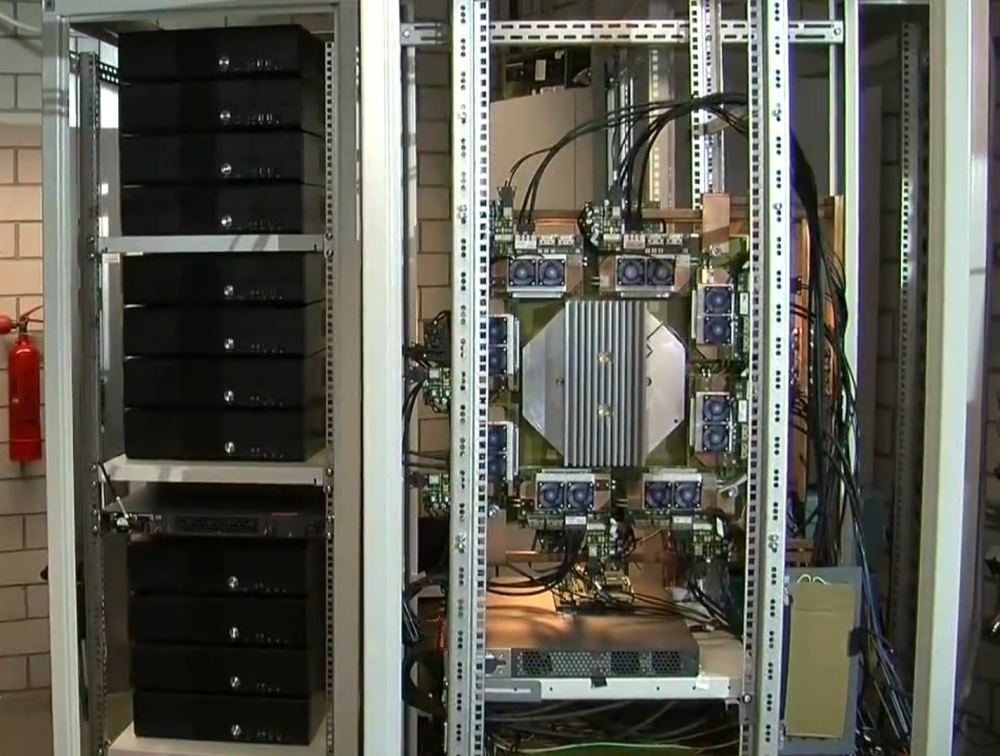
\includegraphics[width=0.5\textwidth]{figures/brainscales}
					
					\caption[The BrainScaleS wafer-scale system.]{The BrainScaleS
					wafer-scale system (right) alongside its supporting conventional PC cluster.}
					
					\label{fig:brainscales}
				\end{figure}
				
				The BrainScaleS project makes use of wafer-scale integration where an
				entire silicon wafer, usually used to manufacture tens or hundreds of
				individual chips, is used as a single system. Instead of slicing the
				wafer into individual reticles, space between the reticles is used to
				build an interconnection network to yield a single large system. A
				system built from a single wafer is able to simulate a network of around
				200,000 neurons up to $10^5$ times faster than biological real-time
				while using 6,000 times less power than a conventional supercomputer
				\cite{schemmel08}.
				
				Each reticle in the wafer contains eight Analog Neural-Network Chips
				(ANCs) which can be programmed to model up to 254 neurons each
				\cite{schemmel10}. There are two types of interconnect between ANCs in
				the system named `level 1' (L1) and `level 2' (L2) which are described
				below.
			
				The L1 network is a mesh network connecting all the ANCs on the same
				wafer together \cite{fieres08}. The network is circuit-switched meaning
				that connecting a set of points in the mesh `uses up' wires along that
				path preventing others from using them. Circuit switched networks offer
				low latency and low-power connections between ANCs compared with a
				packet switched network (more commonly found in modern networks). This
				performance comes at the expense of flexibility as lanes, once
				allocated, cannot be used for any other purpose even when idle. This can
				make changing the connectivity within the network at runtime difficult
				\cite{dally04}, a task required by some learning rules.
				
				Since the L1 network is limited to a single wafer, the L2 network aims
				to work around this limitation. The L2 network is based on 10 gigabit/s
				Ethernet with packets being routed between wafers using off-the-shelf
				network switches and custom FPGA hardware \cite{schemmel10}. This
				network suffers higher latencies than the L1 network but allows signals
				to be routed much more flexibly enabling expansion to multiple wafers
				and other peripherals.  Ethernet (as found in supercomputer networks) is
				also largely optimised for transmission of larger chunks of data.
			
			\subsubsection{Neurogrid}
				
				\begin{figure}
				\end{figure}
				
				\begin{figure}
					\begin{subfigure}[b]{0.49\textwidth}
						\center
						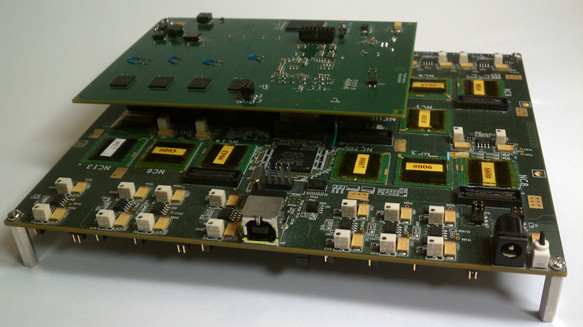
\includegraphics[width=\textwidth]{figures/neurogrid}
						\vspace{0.2cm}
						
						\caption{A 16 chip Nerogrid system.}
						\label{fig:neurogrid}
					\end{subfigure}
					\begin{subfigure}[b]{0.49\textwidth}
						\center
						\begin{tikzpicture}[thick]
	
	\pgfmathsetlengthmacro{\layersep}{-1.3cm}
	\pgfmathsetlengthmacro{\chipsize}{0.8cm}
	
	% A neurocore chip/tree element. Arguments:
	%  #1 ID
	%  #2 Position
	\newcommand{\neurocore}[2]{
		\node (#1) at (#2)
		      [ draw, rectangle
		      , inner sep=0
		      , minimum width =\chipsize
		      , minimum height=\chipsize
		      ]
		      {};
		
		\node (#1 t label) [below      =0 of #1.north]      {\tiny{}T};
		\node (#1 l label) [above right=0 of #1.south west] {\tiny{}L};
		\node (#1 r label) [above left =0 of #1.south east] {\tiny{}R};
		
		\coordinate (#1 t) at (#1 t label.north);
		\coordinate (#1 l) at (#1 l label.south);
		\coordinate (#1 r) at (#1 r label.south);
	}
	
	% FPGA
	\node (fpga) at (3.5, -1*\layersep)
	      [ draw, rectangle
	      , inner sep=0.1cm
	      , minimum width =\chipsize
	      , minimum height=\chipsize
	      ]
	      {\footnotesize{}FPGA};
	
	% Root
	\neurocore{root}{3.5,0*\layersep} \draw (root t) -- (fpga.south);
	
	% Layer 1
	\neurocore{l}{0+1.5,1*\layersep} \draw (l t) -- (root l);
	\neurocore{r}{4+1.5,1*\layersep} \draw (r t) -- (root r);
	
	% Layer 2
	\neurocore{ll}{0+0.5,2*\layersep} \draw (ll t) -- (l l);
	\neurocore{lr}{2+0.5,2*\layersep} \draw (lr t) -- (l r);
	\neurocore{rl}{4+0.5,2*\layersep} \draw (rl t) -- (r l);
	\neurocore{rr}{6+0.5,2*\layersep} \draw (rr t) -- (r r);
	
	% Layer 3
	\neurocore{lll}{0,3*\layersep} \draw (lll t) -- (ll l);
	\neurocore{llr}{1,3*\layersep} \draw (llr t) -- (ll r);
	\neurocore{lrl}{2,3*\layersep} \draw (lrl t) -- (lr l);
	\neurocore{lrr}{3,3*\layersep} \draw (lrr t) -- (lr r);
	\neurocore{rll}{4,3*\layersep} \draw (rll t) -- (rl l);
	\neurocore{rlr}{5,3*\layersep} \draw (rlr t) -- (rl r);
	\neurocore{rrl}{6,3*\layersep} \draw (rrl t) -- (rr l);
	\neurocore{rrr}{7,3*\layersep} \draw (rrr t) -- (rr r);
	
	% Layer 4
	\neurocore{rrrr}{7,4*\layersep} \draw (rrrr t) -- (rrr r);
	
	% USB
	\node (usb) at (3, 4*\layersep)
	      [ draw, rectangle
	      , inner sep=0.1cm
	      , minimum width =\chipsize
	      , minimum height=\chipsize
	      ]
	      {\footnotesize{}USB Interface};
	\draw (usb.north) -- (lrr r);
	
\end{tikzpicture}


						\caption{Neurocores in a 16-chip Neurogrid system.}
						\label{fig:neurogrid-topology}
					\end{subfigure}
					
					\caption{Overview of the Neurogrid architecture.}
					\label{fig:neurogrid-arch-overview}
				\end{figure}
				
				The Neurogrid architecture consists of a tree of 16 `Neurocore' chips.
				Each Neurocore contains a grid of $256 \times 256$ analogue neuron
				models with a modest number of tunable parameters and which run at
				biological real-time. The full 16-Neurocore system can simulate around 1
				million neurons using around three watts \cite{benjamin14}.
				
				When spikes are produced these are transmitted via a digital network to
				all connected neurons\footnote{Neurogrid also features limited tunable
				analogue connectivity for special, local connectivity cases which is not
				discussed here.}. Spikes produced by or destined for a Neurocore are
				streamed one by one to or from the board respectively
				\cite{boahen04,boahen04receiver}.
				
				Neurogrid's analogue neuron models do not account for weighted
				connections so an FPGA is also attached to the network which can be
				configured to probabilistically drop spikes sent via it to a given
				neuron. By altering the probability of spike dropping variable
				connection strengths can be approximated for networks where spike rates,
				but not spike timing, are significant. The Neurogrid tree network also
				includes a USB connection for loading neuron parameters and reading
				results. 
				
				The Neurocore router and its interconnect, described in detail by
				Merolla \emph{et. al.} \cite{merolla14}, is implemented entirely in
				asynchronous logic. Routers communicate on- and off-chip via 1-of-4
				non-return-to-zero links where two electrical transitions are
				required to transmit and acknowledge pairs of two bits. This scheme
				ensures that while idle the router consumes very little power and also
				minimises unnecessary electromagnetic noise which may disrupt sensitive
				analogue neuron circuitry on the chip.
				
				Neurogrid uses multicast wormhole routing allowing the network to easily
				support both large packets during configuration and small packets for
				spike transmission. Wormhole routing allows routers to begin forwarding
				packets immediately rather than storing and then forwarding the whole
				packet. This reduces buffering requirements but also makes it possible
				for the network to deadlock since individual packets can use resources
				in many chips at once and introduce cyclic dependencies \cite{dally04}.
				To avoid deadlock, Neurogrid uses a tree topology as illustrated in
				figure \ref{fig:neurogrid-topology}.  Trees are provably deadlock free
				for unicast traffic and also multicast traffic routed in a specific way.
				
				Since Neurogrid does not use a fat tree topology (described in
				\S\ref{sec:fat-tree}), the network has a throughput bottleneck at the
				root Neurocore's links. The severity of this bottleneck is greatly
				reduced, however, due to the multicast nature of the system. In the
				worst case where all $N$ neurons are connected to every other neuron,
				the throughput requirements of the root node drop from $N^2$ using
				unicast to $N$ for multicast. While this makes the system practical at a
				size of up to 16 Neurocores, if the number of chips were increased, this
				bottleneck would force the use of either higher speed links throughout
				or a change in topology.
			
			
		\subsection{Digital}
			
			% Use digital implementations of neurons, typically optimised in some
			% fashion.
			
			To avoid the difficulties which plague analogue systems, a number of
			researchers have constructed special purpose digital neuron models
			\cite{prange93,jahnke96,schoenauer99,mehrtash03}. Though in principle more
			power efficient and faster than similar software models, these designs are
			inherently tied to a single neural model.
			
			Thanks to the continued gains in power efficiency and speed made by more
			general purpose digital platforms such as CPUs, GPUs and FPGAs, the
			current generation of digital simulators is dominated by these more
			flexible platforms. The mature FPGA-based Bluehive and CPU-based SpiNNaker
			platforms are described below to give an overview of the state of current
			digital simulator technology.
			
			\subsubsection{Bluehive}
				
				% TODO: Include photograph
				\begin{figure} \center
				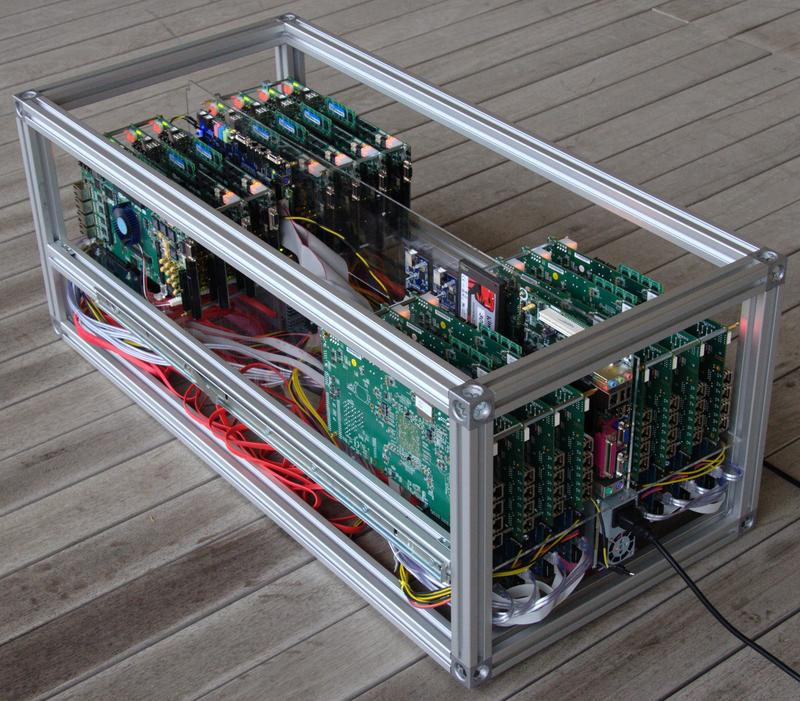
\includegraphics[width=0.4\textwidth]{figures/bluehive}
					
					\caption{A 16 FPGA Bluehive system.} \label{fig:bluehive} \end{figure}
				
				The Bluehive system connects up to 64 high-end Altera Stratix IV FPGAs,
				each simulating up to 64,000 neurons with 1,000 synapses each
				\cite{moore12}. Unlike the analogue systems (and a number of the fixed
				digital systems) which simulate all their neurons in parallel, Bluehive
				multiplexes them four-at-a-time taking advantage of high speed FPGA
				logic. Since duplicating a neuron model will quickly fill an FPGA, it is
				advantageous to implement just a handful of neurons and simply rapidly
				save and restore their state from a large memory bank. In this manner,
				more attention can be spent on making the neuron model fast than making
				it compact. In analogue models, this approach would be impractical
				because analogue state is difficult to save and restore.
				
				The neuron models have been implemented both as custom, special purpose
				hardware and also as conventional C code for a specialised vector
				processor (BlueVec) implemented within the FPGA logic. For the same
				neuron model, a C (software) implementation running on BlueVec required
				an order of magnitude less code than the custom hardware implementation
				yet only performed at half the speed.
				
				The FPGAs are interconnected in a 3D torus ($k$-ary 3-cube) using
				electrical high-speed serial links. A custom protocol is used which
				allows spikes to be reliably transmitted to multiple FPGAs,
				automatically making use alternative connections if a cable is damaged
				or unplugged. The protocol does not, however, include the ability to
				multicast packets to multiple destinations. As a result, a specialised
				`fan-out engine' is used which repeatedly transmits a spike once for
				each destination.
				
				Each of the six bidirectional links are operated at 10 Gbit/s per
				direction and remain powered on in order to ensure low latency
				communication between FPGAs. In practice, each is only loaded on average
				with about 250 MBit/s of traffic which helps reduce congestion in the
				network and thus enable lower latencies.
				
				% TODO: Awaiting some details from Theo about the network.
			
			\subsubsection{SpiNNaker}
				
				% CPU based, custom asynchronous multicast interconnect but scaling up
				% with high-speed serial 2D hexagonal torus network.
				
				% TODO: Refer to this in text.
				\begin{figure}
					\begin{tikzpicture}[thick]
	
	\pgfmathsetlengthmacro{\sep}{2.5em}
	
	\pgfmathsetlengthmacro{\labelsep}{0.5em}
	\tikzset{label/.style={ font=\footnotesize
	                      , align=center
	                      , text width=3cm
	                      , inner sep=0
	                      }}
	
	
	% Callout from #1 to callout box #2 from corner #3 to #4 and corner
	% #5 to #6
	\tikzset{glow/.style={line width=1.0mm,white}}
	\newcommand{\callout}[6]{
		\draw [glow] (#2.north west) rectangle (#2.south east);
		\draw [glow] (#1.#3) -- (#2.#4);
		\draw [glow] (#1.#5) -- (#2.#6);
		
		\draw        (#2.north west) rectangle (#2.south east);
		\draw        (#1.#3) -- (#2.#4);
		\draw        (#1.#5) -- (#2.#6);
	}
	
	\newcommand{\hcallout}[2]{
		\callout{#1}{#2}{north east}{north west}{south east}{south west}
	}
	\newcommand{\vcallout}[2]{
		\callout{#1}{#2}{south east}{north east}{south west}{north west}
	}
	
	% A mess of neurons
	\node (neurons) [inner sep=0]
	      {\input{|"python2 figures/random-network.py 10 25 25 5 0.2 100 3 0.2 1.0"}}
	      ;
	
	% A SpiNNaker die
	\node (die) [inner sep=0]
	      [right=\sep of neurons]
	      {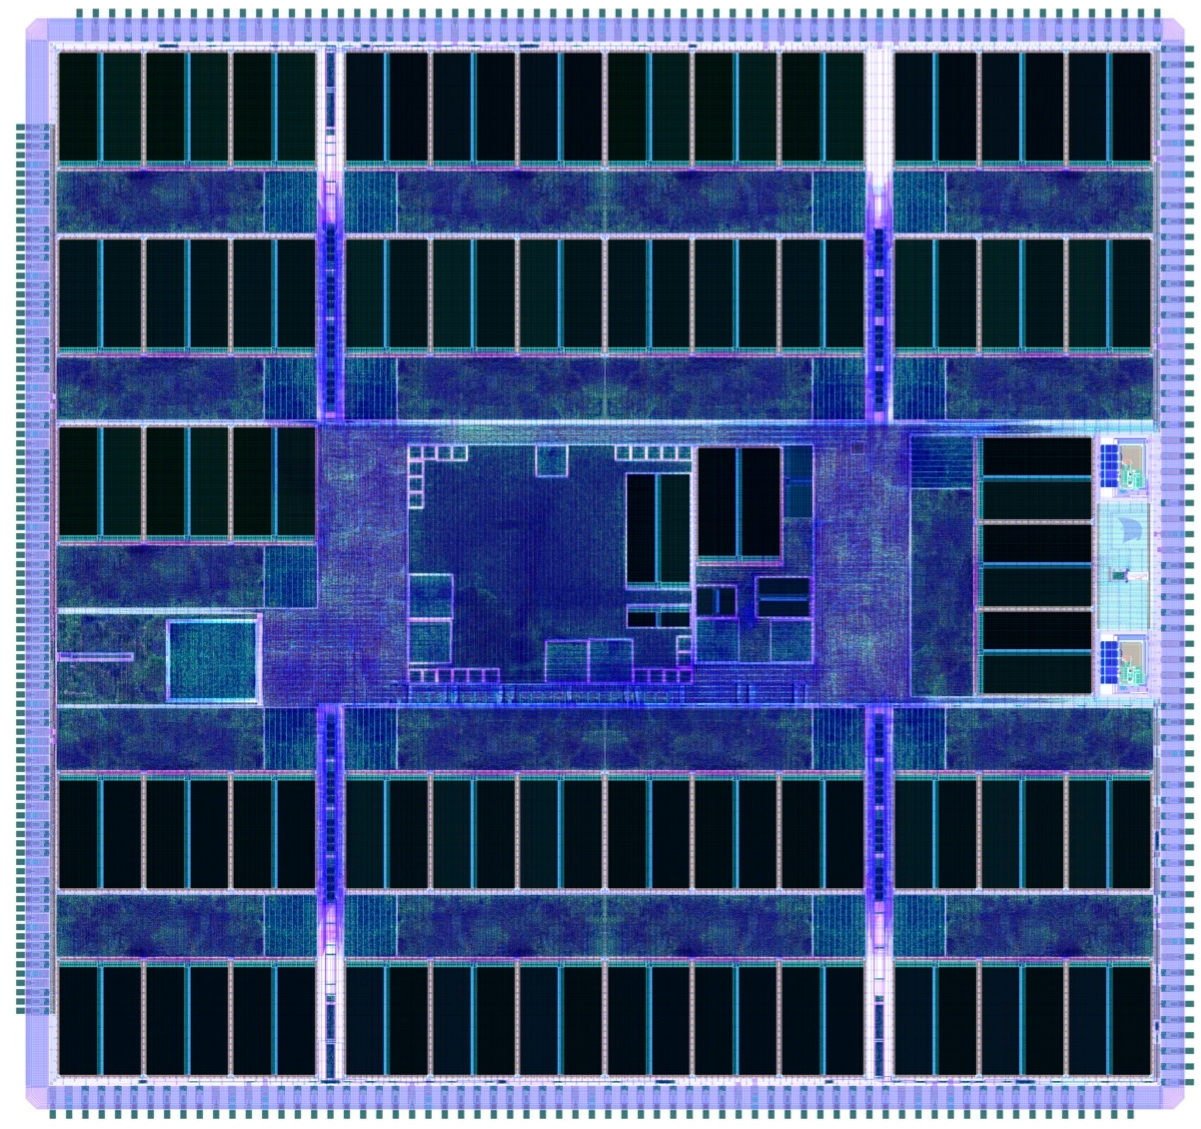
\includegraphics[height=3cm]{figures/spinnakerDie}};
	\node (core) at ([shift={(5.0mm,1.5mm)}]die.west)
	      [ inner sep=0
	      , minimum width =7mm
	      , minimum height=5mm
	      ]
	      {};
	\hcallout{neurons}{core}
	
	% A SpiNNaker board
	\node (board) [inner sep=0]
	      [right=\sep of die]
	      {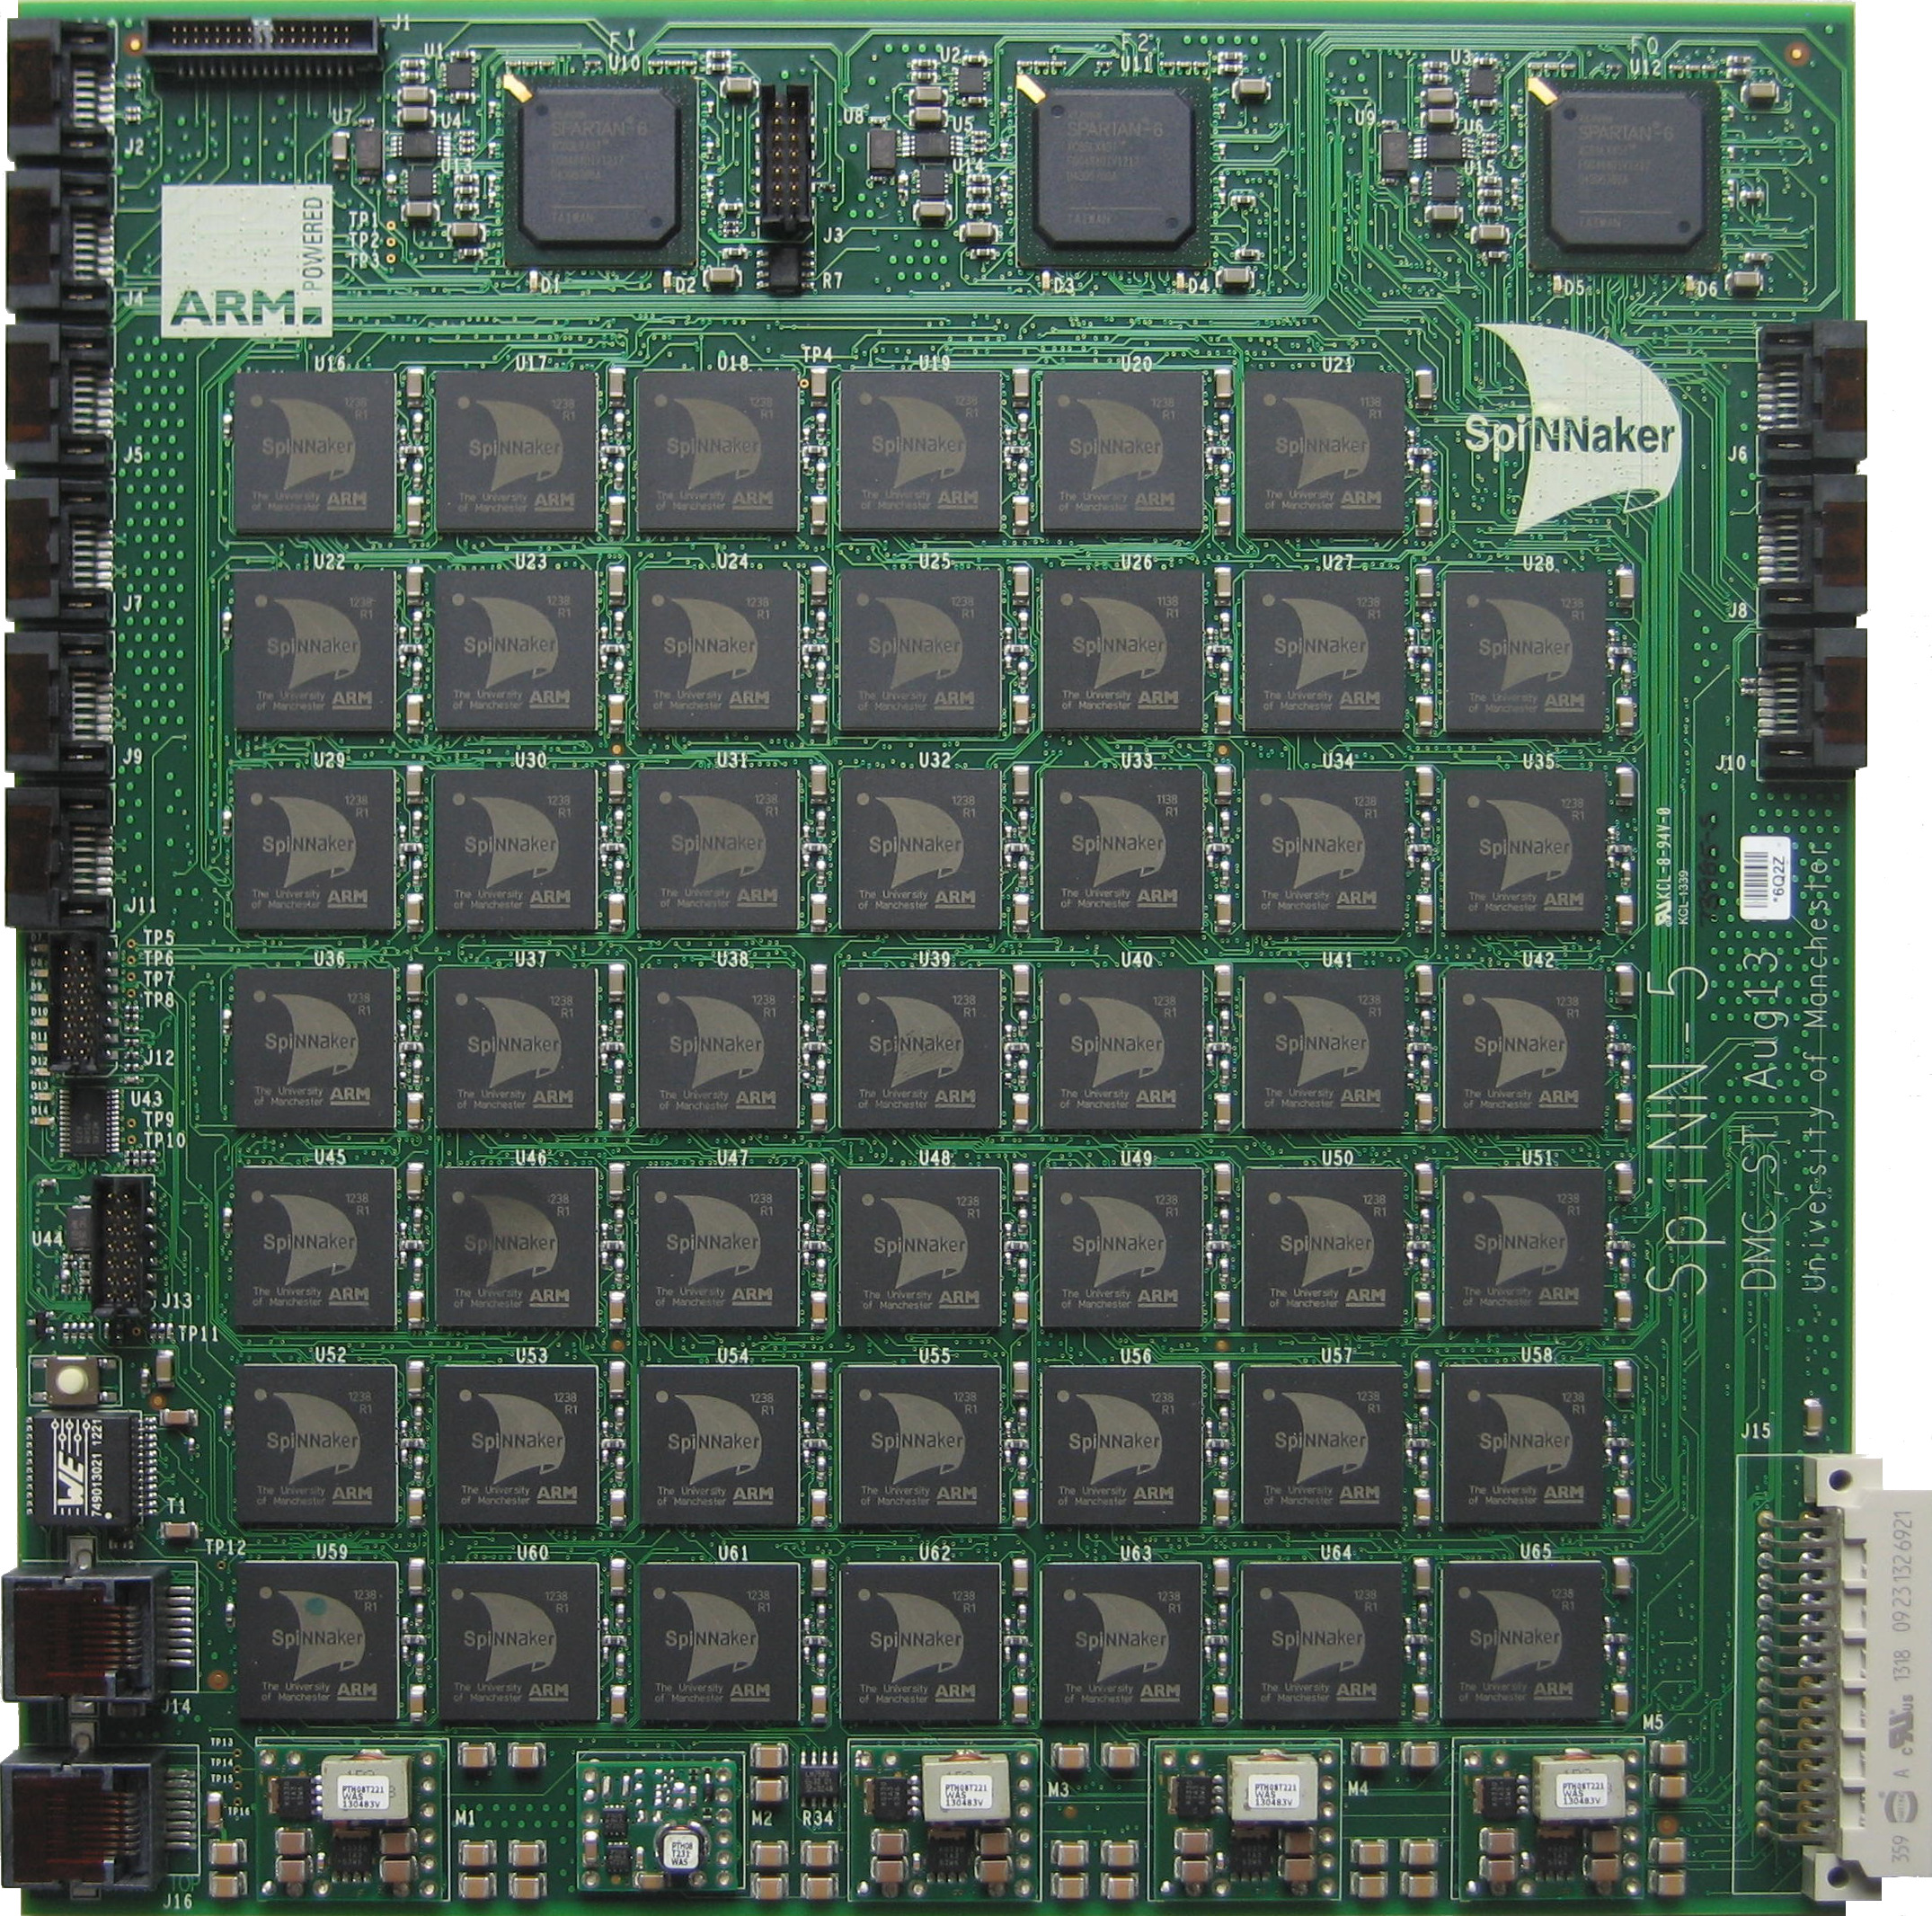
\includegraphics[height=3cm]{figures/spinnakerBoard}};
	\node (chip) at ([shift={(5.0mm,1.6mm)}]board.west)
	      [ inner sep=0
	      , minimum width =3mm
	      , minimum height=3mm
	      ]
	      {};
	\hcallout{die}{chip}
	
	% A rack of boards
	\node (rack) [inner sep=0]
	      [right=\sep of board]
	      {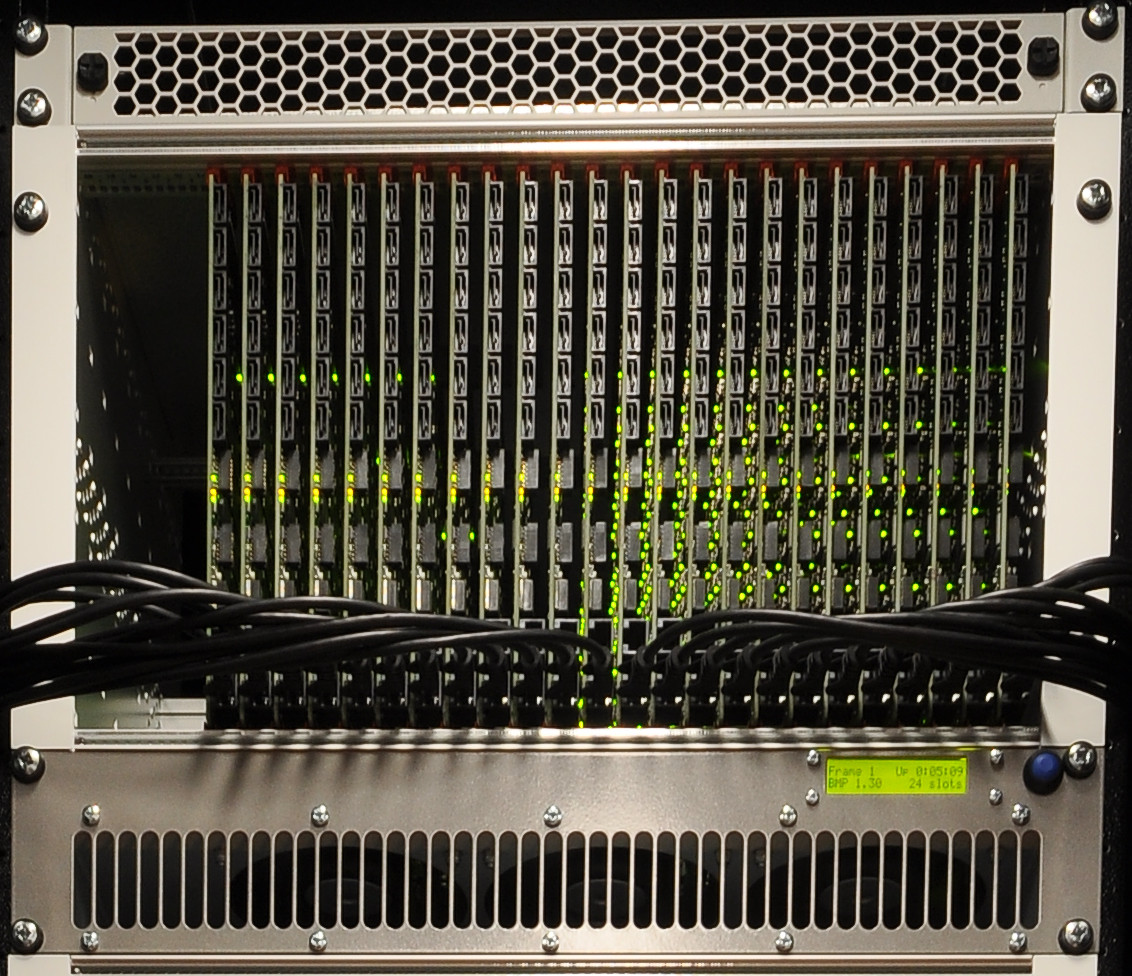
\includegraphics[height=3cm]{figures/spinnakerRack}};
	\node (fitted board) at ([shift={(7mm,2mm)}]rack.west)
	      [ inner sep=0
	      , minimum width =1mm
	      , minimum height=16mm
	      ]
	      {};
	\hcallout{board}{fitted board}
	
	% A ten cabinet machine
	\coordinate (top row) at ($(neurons.south west)!0.5!(rack.south east)$);
	\node (cabinet) [inner sep=0]
	      [below=\sep of top row]
	      {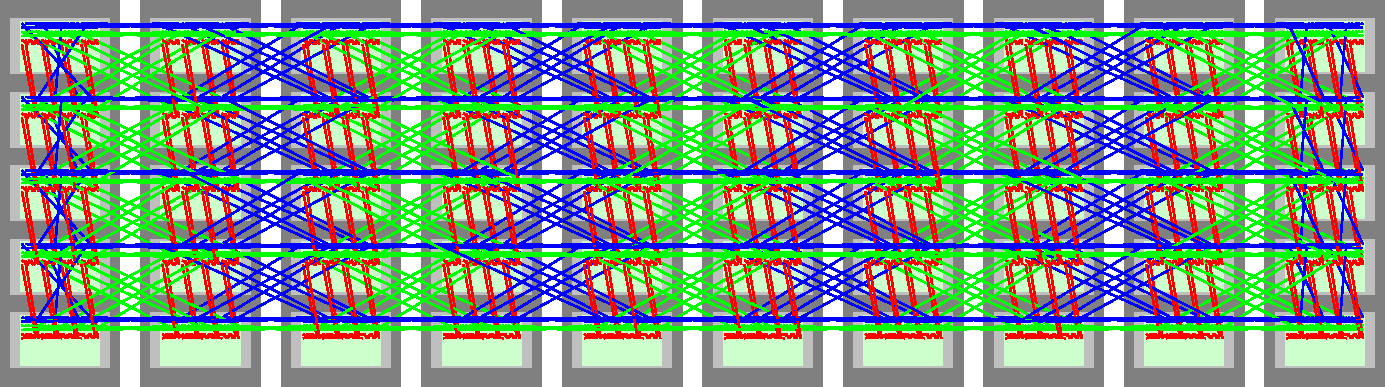
\includegraphics[width=\textwidth]{figures/spinnaker106}};
	\node (fitted rack) at ([shift={(-23.2mm,-5.5mm)}]cabinet.north east)
	      [ inner sep=0
	      , minimum width =11.5mm
	      , minimum height=6.5mm
	      ]
	      {};
	\vcallout{rack}{fitted rack}
	
	% Labels
	\node [above=\labelsep of neurons, label] {1,000 neurons \\ per core.};
	\node [above=\labelsep of die, label] {18 cores \\ per chip.};
	\node [above=\labelsep of board, label] {48 chips \\ per board.};
	\node [above=\labelsep of rack, label] {24 boards \\ per rack.};
	
\end{tikzpicture}


					
					\caption{SpiNNaker hardware abstractions.}
					\label{fig:spinnaker-abstractions}
				\end{figure}
				
				The SpiNNaker architecture consists of a network of up to one million
				low-power mobile-phone grade ARM processors principally interconnected
				using a custom asynchronous network \cite{furber06}. The use of general
				purpose processors allows a great degree of flexibility in the neuron
				implementation at the cost of energy efficiency. 
				
				Figure \ref{fig:spinnaker-abstractions} shows the levels of hardware
				abstraction in SpiNNaker. As in Bluehive, each processor core in
				SpiNNaker is responsible for a number of neurons. The design targets up
				to 1,000 neurons per core each with 1,000 synapses. Eighteen ARM cores
				are combined onto a single SpiNNaker chip which are grouped into boards
				which are assembled into cabinets which will eventually make up a
				machine with 1,036,800 cores capable of simulating around 1 billion
				neurons in biological real time.  At the time of writing, a
				$\frac{1}{10}^{\textrm{th}}$ scale system is being assembled with
				103,680 cores with boards for a full scale system currently being
				manufactured and tested.
				
				\begin{figure}
					\center
							\begin{tikzpicture}[thick,scale=0.80]
			
			\def\width{6}
			\def\height{6}
			\pgfmathtruncatemacro{\widthh}{\width - 1}
			\pgfmathtruncatemacro{\heightt}{\height - 1}
			
			\def\lsize{0.1}
			\def\osize{0.5}
			
			\begin{scope}[minimum size=0.25cm,inner sep=0]
				\foreach \y in {1,...,\height}{
					\foreach \x in {1,...,\width}{
						\node (chip-\x-\y) at (\x,\y) [draw,fill=white,rectangle,minimum size=0.30cm,inner sep=0] {};
					}
				}
			\end{scope}
			
			% The obvious internal links
			\foreach \y in {1,...,\heightt}{
				\foreach \x in {1,...,\widthh}{
					\pgfmathtruncatemacro{\xx}{\x+1}
					\pgfmathtruncatemacro{\yy}{\y+1}
					\draw (chip-\x-\y) -- (chip-\xx-\yy);
					
					\pgfmathtruncatemacro{\xx}{\x+1}
					\pgfmathtruncatemacro{\yy}{\y+0}
					\draw (chip-\x-\y) -- (chip-\xx-\yy);
					
					\pgfmathtruncatemacro{\xx}{\x+0}
					\pgfmathtruncatemacro{\yy}{\y+1}
					\draw (chip-\x-\y) -- (chip-\xx-\yy);
				}
			}
			
			% The non-loop upper/right links
			\foreach \y in {1,...,\heightt}{
				\pgfmathtruncatemacro{\yy}{\y+1}
				\draw (chip-\width-\y) -- (chip-\width-\yy);
			}
			\foreach \x in {1,...,\widthh}{
				\pgfmathtruncatemacro{\xx}{\x+1}
				\draw (chip-\x-\height) -- (chip-\xx-\height);
			}
			
			% The looping left/right links
			\foreach \y in {1,...,\height}{
				\draw 
					(chip-\width-\y) -- ++(\osize,0) arc (-90:90:\lsize);
				\draw  (chip-1-\y) -- ++(-\osize,0) arc (90:-90:-\lsize);
			}
			
			% The looping up/down links
			\foreach \x in {1,...,\width}{
				\draw  (chip-\x-\height) -- ++(0,\osize) arc (180:0:\lsize);
				\draw  (chip-\x-1)       -- ++(0,-\osize) arc (-180:0:\lsize);
			}
			
			% The looping diagonal links
			\foreach \x in {1,...,\width}{
				\draw  (chip-\x-\height) -- ++(\osize,\osize);
				\draw  (chip-\x-1)       -- ++(-\osize,-\osize);
			}
			\foreach \y in {1,...,\height}{
				\draw  (chip-\width-\y) -- ++(\osize,\osize);
				\draw  (chip-1-\y)      -- ++(-\osize,-\osize);
			}
			
		\end{tikzpicture}

					
					\caption[2D hexagonal torus topology used in SpiNNaker.]{2D hexagonal
					torus topology used in SpiNNaker. Each box is an eighteen core
					SpiNNaker chip. Links at the edges of the network wrap-around to
					connect to those on the other side. Actual networks are much larger.}
					\label{fig:spinn-topology}
				\end{figure}
				
				Chips are connected in a 2D hexagonal torus topology, illustrated in
				figure \ref{fig:spinn-topology}, using a combination of custom
				asynchronous interconnect between chips on the same circuit board (as in
				Neurogrid) and high-speed serial between boards (as in Bluehive).
				
				Unlike Neurogrid and Bluehive, the SpiNNaker network is potentially
				vulnerable to deadlock when heavily congested. To reduce the risk of
				this occurring, the network is over-provisioned such that during
				expected operation it should be lightly loaded. Additionally, if a
				deadlock occurs, it is broken using a simple packet dropping mechanism
				when a packet has taken too long to progress. Though this means packet
				delivery is not guaranteed, it assumed that likelihood of this occurring
				is low and that neural networks are inherently tolerant to the rare loss
				of spikes, as observed in biology. For networks where guaranteed
				delivery is desired, dropped packets are not actually lost, instead
				they're copied into a buffer where user software is able to reinject
				them at an appropriate moment.
	
	\section{SpiNNaker network architecture}
		\label{sec:spinnaker}
		
		% Greater detail intro to SpiNNaker since it will be the focus of this work
		%
		% Overview of system: cores, chips, boards, racks, cabinets. Network is
		% hexagonal torus with nodes being chips.
		
		This section gives a more detailed overview of SpiNNaker's network
		architecture which forms the focus of current preliminary work and a
		platform for future work. In particular, the section outlines the format of
		packets within the network and the methods by which they are routed. The
		section concludes with a description of the link technology from which the
		network is implemented.
		
		\subsection{SpiNNaker packets}
			
			% Packet types and sizes. Table based routing, generally, multicast
			% routing in SpiNNaker. Also describe the sort of fun which can be had
			% with multicast, mention power savings due to less hops. Mention router
			% simplicity, limitations, assumptions.
			
			\begin{figure}
				\center
				\begin{tikzpicture}[ thick
                   , blockstyle/.style={ draw
                                       , rectangle
                                       , minimum height=2em
                                       }
                   ]
	\pgfmathsetlengthmacro{\bitlen}{0.5em}
	\pgfmathsetlengthmacro{\bitdashlen}{0.3em}
	
	% #1: Node to draw on
	% #2: Number of bits
	\newcommand{\bitdashes}[2]{
		\pgfmathsetmacro{\boundaries}{#2-1}
		\begin{scope}[help lines]
			\foreach \x in {1,...,\boundaries}{
				\draw ([shift={(\x*\bitlen,0)}] #1.north west)
				   -- ++(0, -\bitdashlen);
				
				\draw ([shift={(\x*\bitlen,0)}] #1.south west)
				   -- ++(0, \bitdashlen);
			}
		\end{scope}
		
		\draw [ decorate
		      , decoration={ brace
		                   , amplitude=1ex
		                   , raise=0.2ex
		                   }
		      ]
		      (#1.south east)
		   -- node [anchor=north, yshift=-1.2ex] {#2 bits}
		      (#1.south west);
	}
	
	\node (control)
	      [ blockstyle
	      , minimum width=8*\bitlen
	      ]
	      {control};
	\bitdashes{control}{8}
	
	\node (key)
	      [ blockstyle
	      , minimum width=32*\bitlen
	      , right=-\the\pgflinewidth of control
	      ]
	      {key};
	\bitdashes{key}{32}
	
	\node (payload)
	      [ blockstyle
	      , minimum width=32*\bitlen
	      , right=-\the\pgflinewidth of key
	      ]
	      {optional payload};
	\bitdashes{payload}{32}
	
\end{tikzpicture}


				
				\caption{SpiNNaker multicast packet format.}
				\label{fig:spinnaker-packet}
			\end{figure}
			
			Cores within SpiNNaker are able to communicate through the transmission of
			small `SpiNNaker packets'. These packets are either 40 or 72 bits long and
			are designed primarily for the efficient communication of neural spikes.
			Though a number of types of packet exist for system configuration
			purposes, applications typically communicate using multicast packets which
			are formatted as shown in figure \ref{fig:spinnaker-packet}. The `control'
			field essentially indicates the type of packet. The `key' (interchangeably
			referred to as `routing key') field is specified by the application and is
			used to route the packet through the system. Finally, an optional
			`payload' field can be added by applications that require it.
			
			In typical spiking neural applications the payload field isn't required
			meaning that all packets sent are only 40 bits long. A neural spike event
			contains only two pieces of information: the identity of the neuron that
			fired and the time that it occurred. Since SpiNNaker operates in real-time
			and the network is designed to deliver packets within a single simulation
			time-step, the time of the spike is implied by the time of the packets'
			arrival. This simply leaves the neuron's identity which is also used as a
			routing key \cite{davies12}.
		
		\subsection{Routing}
			
			\label{sec:spinn-router}
			
			One of the key features of SpiNNaker's network is its support for
			multicast routing of packets. Packets are forwarded around the network by
			the router included in each eighteen core SpiNNaker chip. When a multicast
			packet arrives at a router, it looks up the key in a routing table to
			select a set of destinations for the packet. The router can forward
			packets to any combination of routers on neighbouring chips and to each of
			the eighteen local cores. By configuring the routing tables appropriately,
			spikes produced by the simulated neurons can be forwarded and multicast to
			every core in which they're required.
			
			Since the system is designed to deal with up to a billion neurons, the
			number of routing table entries required to explicitly route every spike
			would be prohibitive. To reduce the number of routing entries required, a
			number of simple compression techniques are required.
			
			The first compression technique is that in most neural simulations, spikes
			from every neuron in a particular population of neurons are typically
			routed identically. To exploit this, routing keys may be split into two
			parts: one which identifies the population from which a spike originates
			and a another which identifies the exact neuron within that population.
			By configuring the router to only compare the routing key against the part
			which indicates the population, a single routing entry can be used for an
			entire population. Since populations may contain thousands of neurons,
			this technique substantially reduces the number of entries required.
			
			To implement this first compression technique, each entry in the routing
			table contains a key, mask and destination field. The mask field can be
			used to ignore the bits in a packet's key, for example those which
			correspond to specific neurons within a population. If the packet's masked
			key matches the key in the table entry, it is routed according to the
			destination field. Using a hardware device called a ternary Content
			Addressable Memory (CAM), this masking and comparison operation can be
			performed for every entry in a routing table in a single clock cycle.
			
			A second compression technique exploits the regular structure of the
			network's topology. If packets are due to travel along a straight line in
			the network without changing direction, routing entries are only required
			for routers where the packet enters the network, changes direction or is
			delivered to a core. Specifically, if a router receives a packet for which
			no routing entry matches, `default' routing is used where the packet is
			forwarded to the link opposite the one it entered. For example, a packet
			arriving on the North link would be forwarded to the South link. This
			technique makes it possible to construct routes where the number of
			routing entries required is $\le 1 + 2D$ where $D$ is the number of
			destinations, no matter how far apart the source and destinations of the
			route are.
			
			As a result of these compression techniques, SpiNNaker's routing tables
			contain 1,024 entries which is hoped to be sufficient for very large
			networks.
		
		\subsection{Link technologies}
			
			% Between and within chips use asynchronous links. Between boards this
			% would be impractical due to number of wires and performance over long
			% wires. Instead, high-speed serial via FPGAs is used. Minimal torus
			% construction.
			
			\begin{figure}
				\begin{subfigure}[b]{0.49\textwidth}
					\center
					\begin{tikzpicture}[thick,scale=0.3,inner sep=0]
	\begin{scope}[hexagonXYZ]
		\foreach \xoff/\yoff/\colour in {%
			0/0/red,%
			4/8/green,%
			8/4/blue%
		}{
			\foreach \x/\y/\num in {%
			                                          0/4/45,   1/4/46,   2/4/47,   3/4/48, %
			                                -1/3/44,  0/3/25,   1/3/26,   2/3/27,   3/3/28, %
			                      -2/2/43,  -1/2/24,  0/2/11,   1/2/12,   2/2/13,   3/2/29, %
			            -3/1/42,  -2/1/23,  -1/1/10,  0/1/3,    1/1/4,    2/1/14,   3/1/30, %
			  -4/0/41,  -3/0/22,  -2/0/9,   -1/0/2,   0/0/1,    1/0/5,    2/0/15,   3/0/31, %
			  -4/-1/40, -3/-1/21, -2/-1/8,  -1/-1/7,  0/-1/6,   1/-1/16,  2/-1/32,          %
			  -4/-2/39, -3/-2/20, -2/-2/19, -1/-2/18, 0/-2/17,  1/-2/33,                    %
			  -4/-3/38, -3/-3/37, -2/-3/36, -1/-3/35, 0/-3/34,                              %
			}{
			  \node [draw,hexagon,minimum size=0.3cm,inner sep=0,font=\footnotesize,\colour]
			        at (\x+\xoff,\y+\yoff) (chip \num) {};
			}
		}
	\end{scope}
	
\end{tikzpicture}

					
					\caption{Tiling of three boards.\color{white}{\\~}}
					\label{fig:threeboard}
				\end{subfigure}
				\begin{subfigure}[b]{0.49\textwidth}
					\center
					\begin{tikzpicture}[thick,scale=0.3,inner sep=0]
	\begin{scope}[hexagonXYZ]
		\foreach \xoff/\yoff/\colour in {%
			0/0/red,%
			4/8/green,%
			8/4/blue%
		}{
			\foreach \x/\y/\num in {%
			                                          0/4/45,   1/4/46,   2/4/47,   3/4/48, %
			                                -1/3/44,  0/3/25,   1/3/26,   2/3/27,   3/3/28, %
			                      -2/2/43,  -1/2/24,  0/2/11,   1/2/12,   2/2/13,   3/2/29, %
			            -3/1/42,  -2/1/23,  -1/1/10,  0/1/3,    1/1/4,    2/1/14,   3/1/30, %
			  -4/0/41,  -3/0/22,  -2/0/9,   -1/0/2,   0/0/1,    1/0/5,    2/0/15,   3/0/31, %
			  -4/-1/40, -3/-1/21, -2/-1/8,  -1/-1/7,  0/-1/6,   1/-1/16,  2/-1/32,          %
			  -4/-2/39, -3/-2/20, -2/-2/19, -1/-2/18, 0/-2/17,  1/-2/33,                    %
			  -4/-3/38, -3/-3/37, -2/-3/36, -1/-3/35, 0/-3/34,                              %
			}{
				\pgfmathtruncatemacro{\xx}{\x+\xoff}
				\pgfmathtruncatemacro{\yy}{\y+\yoff}
				\ifthenelse{\xx < 0}{
					\pgfmathtruncatemacro{\xx}{\xx+12}
				}{}
				\ifthenelse{\yy > 8}{
					\pgfmathtruncatemacro{\yy}{\yy-12}
				}{}
				\node [draw,hexagon,minimum size=0.3cm,inner sep=0,font=\footnotesize,\colour]
				      at (\xx,\yy) (chip \num) {};
			}
		}
	\end{scope}
	
\end{tikzpicture}

					\vspace{0.5cm}
					
					\caption{Redrawn to show torus. Wrap-around connections connect
					opposing edges (not shown).}
					\label{fig:threeboard-sliced}
				\end{subfigure}
				
				\caption[Minimal tiling of three SpiNNaker forming a torus.]{Minimal
				tiling of three SpiNNaker forming a torus. Hexagons represent SpiNNaker
				chips on a board and the colour indicates which board a chip belongs
				to.}
				\label{fig:spinnaker-tiling}
			\end{figure}
			
			SpiNNaker chips are assembled on to boards of 48 chips. The chips on each
			board are logically connected into a hexagonal shape which allows boards
			to be tiled as shown in figure \ref{fig:threeboard}. Connections must then
			be made between chips on neighbouring boards to complete the network. The
			three boards shown can be further connected to form a torus, a process
			which is more clearly visualised in figure \ref{fig:threeboard-sliced}. By
			repeating this pattern, arbitrarily large torus networks can be
			constructed using 48 chip boards.
			
			Between individual SpiNNaker chips, an asynchronous `2-of-7' protocol is
			used to communicate packets. This system enables low-power communication
			between chips which only uses power during data transmission.
			Unfortunately, 2-of-7 codes use sixteen electrical signals (eight per
			direction) for each chip-to-chip link. Though this is acceptable for chips
			sharing a circuit board where wires are relatively cheap, connecting the
			768 wires to other boards is not practical. As a result, six bundles of
			eight chip-to-chip links each are transparently multiplexed/demultiplexed
			onto six high-speed serial (HSS) links, one for each bundle. These links
			(described in greater detail in the next section) require only two signals
			but operate more than eight times faster than the 2-of-7 links and so no
			throughput penalty is incurred.
			
			The HSS links are implemented within the three FPGAs present in each 48
			chip SpiNNaker board. Each FPGA independently handles two of the HSS
			board-to-board links. These FPGAs also feature additional connectivity
			which are aimed to be exploited as part of the work proposed in this
			report.
	
	\section{High-Speed Serial (HSS)}
		\label{sec:high-speed-serial}
		
		% Technology now used by most supercomputers and high-speed comms tasks.
		% More complex than parallel but they scale up throughput better.
		
		\begin{figure}
			\begin{subfigure}{0.48\textwidth}
				\center
				\begin{tikzpicture}[thick, node distance=0.2cm, xscale=0.40]
					% #1: Name of waveform
% #2: Text label for waveform
% #3: Style (e.g. below=of) of waveform
% #4: List of waveform values
% #5: Offset
% #6: Maximum Offset
% #7: First bit value
\newcommand{\waveform}[7]{
	% Label
	\node (#1) [#3] {#2};
	
	% Draw the leading line
	\draw (#1.east) -- ++(#5,0)
	      coordinate (last wave point)
	      ;
	
	% Draw the waveform
	\foreach [count=\i] \bit in {#4}{
		
		\ifthenelse{\equal{\bit}{1}}{
			\draw let \p1=(last wave point)
			        , \p2=(#1.north east)
			   in (last wave point)
			   -- (\x1,\y2)
			   -- ++(1,0)
			      coordinate (last wave point)
			      ;
		}{
			\draw let \p1=(last wave point)
			        , \p2=(#1.south east)
			   in (last wave point)
			   -- (\x1,\y2)
			   -- ++(1,0)
			      coordinate (last wave point)
			      ;
		}
	}
	
	% Finish the line
	\draw let \p1=(last wave point)
	        , \p2=(#1.east)
	   in (last wave point)
	   -- (\x1,\y2)
	   -- ++(2-#5,0)
	      coordinate (last wave point)
	      ;
	
	% Draw an arrow indicating offset
	\pgfmathsetlengthmacro{\absoffset}{abs(#5cm - #6cm - 0.5cm/2)}
	\ifthenelse{\equal{#6}{0.000000} \or \lengthtest{\absoffset < 0.2cm}}{
		% No offset...
	}{
		% Get vertical position
		\ifthenelse{\equal{#7}{1}}{
			\coordinate (offset arrow ypos) at (#1.south east);
		}{
			\coordinate (offset arrow ypos) at (#1.north east);
		}
		\coordinate (offset arrow ypos) at ($(offset arrow ypos)!0.5!(#1.east)$);
		
		\ifthenelse{\lengthtest{#5cm > #6cm/2}}{
			\draw [red,->] ([shift={(0.3,0)}]offset arrow ypos -| #1.east) -- ++(0.7,0);
		}{
			\draw [red,<-] ([shift={(0.3,0)}]offset arrow ypos -| #1.east) -- ++(0.7,0);
		}
	}
	
}

					\input{|"python figures/parallel_example.py 'Hello, World!' 0.0"}
					
				\end{tikzpicture}
				
				\caption{No skew.}
				\label{fig:parcons-no-skew}
			\end{subfigure}
			\begin{subfigure}{0.48\textwidth}
				\center
				\begin{tikzpicture}[thick, node distance=0.2cm, xscale=0.40]
					% #1: Name of waveform
% #2: Text label for waveform
% #3: Style (e.g. below=of) of waveform
% #4: List of waveform values
% #5: Offset
% #6: Maximum Offset
% #7: First bit value
\newcommand{\waveform}[7]{
	% Label
	\node (#1) [#3] {#2};
	
	% Draw the leading line
	\draw (#1.east) -- ++(#5,0)
	      coordinate (last wave point)
	      ;
	
	% Draw the waveform
	\foreach [count=\i] \bit in {#4}{
		
		\ifthenelse{\equal{\bit}{1}}{
			\draw let \p1=(last wave point)
			        , \p2=(#1.north east)
			   in (last wave point)
			   -- (\x1,\y2)
			   -- ++(1,0)
			      coordinate (last wave point)
			      ;
		}{
			\draw let \p1=(last wave point)
			        , \p2=(#1.south east)
			   in (last wave point)
			   -- (\x1,\y2)
			   -- ++(1,0)
			      coordinate (last wave point)
			      ;
		}
	}
	
	% Finish the line
	\draw let \p1=(last wave point)
	        , \p2=(#1.east)
	   in (last wave point)
	   -- (\x1,\y2)
	   -- ++(2-#5,0)
	      coordinate (last wave point)
	      ;
	
	% Draw an arrow indicating offset
	\pgfmathsetlengthmacro{\absoffset}{abs(#5cm - #6cm - 0.5cm/2)}
	\ifthenelse{\equal{#6}{0.000000} \or \lengthtest{\absoffset < 0.2cm}}{
		% No offset...
	}{
		% Get vertical position
		\ifthenelse{\equal{#7}{1}}{
			\coordinate (offset arrow ypos) at (#1.south east);
		}{
			\coordinate (offset arrow ypos) at (#1.north east);
		}
		\coordinate (offset arrow ypos) at ($(offset arrow ypos)!0.5!(#1.east)$);
		
		\ifthenelse{\lengthtest{#5cm > #6cm/2}}{
			\draw [red,->] ([shift={(0.3,0)}]offset arrow ypos -| #1.east) -- ++(0.7,0);
		}{
			\draw [red,<-] ([shift={(0.3,0)}]offset arrow ypos -| #1.east) -- ++(0.7,0);
		}
	}
	
}

					\input{|"python figures/parallel_example.py 'Hello, World!' 0.7"}
					
				\end{tikzpicture}
				
				\caption{With skew.}
				\label{fig:parcons-with-skew}
			\end{subfigure}
			
			\caption[Parallel signalling example.]{Example of parallel data
			transmission. Eight bits are transferred each cycle and the value of the
			signals sampled at the point indicated by the faint line. As skew is
			introduced, errors appear.}
			\label{fig:parcons} \end{figure}
		
		Traditionally, digital links within computers have relied on parallel
		signalling where a `word' consisting of multiple bits is transmitted
		simultaneously each clock tick (figure \ref{fig:parcons-no-skew}). This
		mechanism is popular because it is simple and allows easy scaling by simply
		increasing the number of bits within in a word. Unfortunately, as the speed
		at which devices run increases, the assumption that the times taken by
		signals to propagate down different wires is the same has fallen apart. This
		`skew' between signals means that a receiver may erroneously receive bits
		from different words at the same time on different wires resulting in an
		error (figure \ref{fig:parcons-with-skew}). Though skew can be minimised by
		matching the quality and lengths of the wires used, this is expensive and
		does not scale well.
		
		Serial signalling, by contrast, only transmits one bit at a time thus
		avoiding skew related issues. In addition, serial signalling reduces the
		number of physical wires required to transmit data. Since the number of
		connections required by a chip or circuit board can have a large influence
		on cost, this factor alone may make serial a necessary choice.
		
		While low-speed serial signalling techniques such as RS232 can be extremely
		simple, at higher speeds matters become more complex. This section describes
		a number of the techniques employed by high-speed serial links and their
		implications for interconnection networks. A more in-depth treatment of HSS
		technology can be found by Athavale \emph{et. al.} \cite{athavale05}.
		
		\subsection{Clock recovery}
			
			% Requires frequent transitions (e.g. using 8b/10b) even on idle line,
			% makes idling expensive.
			
			Since serial signals can only transmit a single bit per clock cycle, to
			achieve high bandwidths HSS links typically operate at multiple gigahertz.
			Transmitting this clock signal alongside the data would require a large
			amount of power and be electrically challenging to connect due to the need
			to minimise skew between the data and clock signals.
			
			An alternative to transmitting the clock signal is to extract the clock
			from the data stream itself. This is typically done using a Clock Recovery
			Circuit (CRC). This circuit can derive a clock signal from an incoming
			data stream if the data features frequent enough transitions between 0 and
			1. To guarantee this, data sent down the link must be encoded using a
			scheme such as 8b/10b coding \cite{widmer83} which translates arbitrary
			eight bit values and encodes these at ten bit sequences with guaranteed
			frequent transitions.
			
			The need for frequent transitions also implies that the link must
			constantly transmit values in order for the clock to be reconstructed by
			the receiver. Further, it takes some time for a CRC to lock onto the clock
			used by an incoming stream of data. These properties can have a
			significant impact on the power consumption of serial links over which low
			latency communication is required.
		
		\subsection{Clock correction}
			
			High-speed serial links are typically designed to allow communication
			between two devices each using their own independent clock source to
			transmit data. This causes problems since no two clocks run at exactly the
			same speed meaning that a faster device will send slightly more data than
			the slower device can handle. For a clock with with an error of 100 Parts
			Per Million (PPM), this means that, in the worst case, in the time it
			takes a fast device to transmit 10,001 bits, a slow device would only be
			able to process 9,999 bits.
			
			Though a receiver is able to derive the clock used by the sender, this
			clock is typically only used to place the data from the incoming serial
			steam into a FIFO buffer. Data placed in this buffer is then read by the
			receiving system using its own clock. Unfortunately, this buffer will
			inevitably overflow or underflow depending on the relative speed of the
			sender's clock. One of the additional features provided by 8b/10b coding
			is the provision of a number `out-of-band' codes, known as K-characters,
			which do not correspond to any eight bit sequence. To avoid buffer
			under/overflow, senders periodically insert a `skip sequence' of a number
			of K-characters.  If the receiver's clock is running slower than the
			sender's, its buffer will gradually fill up. If the buffer fills beyond a
			high-water mark, the receiver will drop any skip sequences it receives
			allowing it to catch up and the buffer to empty. Conversely, if the
			receiver is faster than the sender, its buffer will gradually empty.  If a
			low-water mark is passed, the receiver may duplicate any skip sequences in
			its buffer. As a side-effect of this behaviour, a certain amount of
			buffering is required by HSS systems which contributes both to chip area
			requirements and latency involved in traversing a link.
		
		\subsection{Error recovery}
			
			No link technology is perfectly reliable with HSS being no exception and
			thus is susceptible to occasional bit errors. As a result, an error
			detection and recovery mechanism must be used to ensure reliable delivery
			of data.
			
			In noisy communication systems such as wireless networks where bit errors
			are frequent forward error correction (FEC) is used which redundantly
			encodes data such that it is still recoverable in the presence of certain
			errors.  HSS links are typically far less noisy and thus errors are
			comparatively rare.  In order to avoid the significant communication and
			computation overhead involved in FEC, HSS links typically use checksums to
			detect the validity of arriving data and a resend mechanism to request
			retransmission when corrupted data arrives.
			
			Resend mechanisms require that senders retain copies of data due to be
			sent over a link until it is acknowledged as successfully received by the
			receiver. The number of packets which must be retained is determined by
			the frequency with which acknowledgements are sent for correctly arriving
			data. The overheads introduced by transmitting acknowledgements along with
			the buffering used are parameters that must be tuned to for a given
			application. These overheads typically are far less significant than those
			added by FEC when the number of errors is low. Retransmission does,
			however, add significantly to the latency cost of errors since a
			round-trip delay is incurred in the sending of a negative acknowledgement
			and awaiting retransmission.
		
		\subsection{Flow control}
			
			Finally, due to the amount of buffering required for a HSS link, flow
			control cannot be as simple as a handshaking mechanism where blocks of
			data are individually acknowledged or blocked since waiting for these
			signals would introduce a large overhead. As a result, more sophisticated
			schemes such as credit based flow control \cite{dally04} may be used.
			These mechanisms introduce additional complexity and buffering by
			typically only a minimal latency penalty.
